\documentclass[xetex,mathserif,serif]{beamer}
\usepackage{polyglossia}
\setdefaultlanguage[babelshorthands=true]{russian}
\usepackage{minted}
\usepackage{tabu}

\useoutertheme{infolines}

\usepackage{fontspec}
\setmainfont{FreeSans}
\newfontfamily{\russianfonttt}{FreeSans}

\setbeamertemplate{blocks}[rounded][shadow=false]
\setbeamercolor*{block title example}{fg=green!50!black,bg=green!20}
\setbeamercolor*{block body example}{fg=black,bg=green!10}

\setbeamercolor*{block title alerted}{fg=red!50!black,bg=red!20}
\setbeamercolor*{block body alerted}{fg=black,bg=red!10}

\tabulinesep=0.7mm

\title{Задача про систему контроля версий}
\author[Юрий Литвинов]{Юрий Литвинов \newline \textcolor{gray}{\small\texttt{yurii.litvinov@gmail.com}}}

\date{02.03.2017г}

\begin{document}
	
	\frame{\titlepage}
	
	\section{Разбор домашки про Lazy}

	\begin{frame}[fragile]
		\frametitle{Double-checked locking}
		Вот так неправильно:
		\begin{minted}{java}
private T value;

T get() {
    if (value == NONE) {
        synchronized (this) {
            if (value == NONE) {
                value = supplier.get();
            }
        }
    }
    return value;
}
		\end{minted}
\end{frame}

	\begin{frame}[fragile]
		\frametitle{Double-checked locking}
		Вот так правильно (начиная с Java 5):
		\begin{minted}{java}
private volatile T value;

T get() {
    if (value == NONE) {
        synchronized (this) {
            if (value == NONE) {
                value = supplier.get();
            }
        }
    }
    return value;
}
		\end{minted}
\end{frame}

	\begin{frame}[fragile]
		\frametitle{Double-checked locking}
		Или даже так:
		\begin{minted}{java}
private volatile T value;

T get() {
    T result = value;
    if (result == NONE) {
        synchronized (this) {
            result = value;
            if (result == NONE) {
                result = value = supplier.get();
            }
        }
    }
    return result;
}
		\end{minted}
\end{frame}

	\begin{frame}[fragile]
		\frametitle{Lock-free}
		\begin{minted}{java}
T get() {
    if (value == NONE) {
        Supplier<T> local = supplier;
        if (local != null) {
            if (updater.compareAndSet(this, NONE, local.get())) {
                supplier = null;
            }
        }
    }
    return value;
}}
		\end{minted}
\end{frame}

	\section{Внутреннее устройство Git}

	\begin{frame}
		\frametitle{Немного про внутреннее устройство Git\footnote{\tiny{По гл. 10 \url{https://git-scm.com/book} и \url{http://aosabook.org/en/git.html}}}}
		Структура папки .git:
		\begin{itemize}
			\item HEAD
			\item index
			\item config
			\item description
			\item hooks/
			\item info/
			\item objects/
			\item refs/
			\item ...
		\end{itemize}
	\end{frame}

	\begin{frame}[fragile]
		\frametitle{Объекты}
		Git внутри --- хеш-таблица, отображающая SHA-1-хеш файла в содержимое файла. Пример:
		\begin{minted}{text}
$ git init test
Initialized empty Git repository in /tmp/test/.git/
$ cd test
$ find .git/objects
.git/objects
.git/objects/info
.git/objects/pack

$ echo 'test content' | git hash-object -w --stdin
d670460b4b4aece5915caf5c68d12f560a9fe3e4

$ find .git/objects -type f
.git/objects/d6/70460b4b4aece5915caf5c68d12f560a9fe3e4
		\end{minted}
\end{frame}

	\begin{frame}[fragile]
		\frametitle{Объекты (2)}
		Как получить сохранённый объект:
		\begin{minted}{text}
$ git cat-file -p d670460b4b4aece5915caf5c68d12f560a9fe3e4
test content
		\end{minted}

		Версионный контроль:
		\begin{minted}{text}
$ echo 'version 1' > test.txt
$ git hash-object -w test.txt
83baae61804e65cc73a7201a7252750c76066a30
$ echo 'version 2' > test.txt
$ git hash-object -w test.txt
1f7a7a472abf3dd9643fd615f6da379c4acb3e3a
$ find .git/objects -type f
.git/objects/1f/7a7a472abf3dd9643fd615f6da379c4acb3e3a
.git/objects/83/baae61804e65cc73a7201a7252750c76066a30
.git/objects/d6/70460b4b4aece5915caf5c68d12f560a9fe3e4
		\end{minted}
\end{frame}

	\begin{frame}[fragile]
		\frametitle{Объекты (3)}
		Переключение между версиями файла:
		\begin{minted}{text}
$ git cat-file -p 83baae61804e65cc73a7201a7252750c76066a30 \
    > test.txt
$ cat test.txt
version 1

$ git cat-file -p 1f7a7a472abf3dd9643fd615f6da379c4acb3e3a \
    > test.txt
$ cat test.txt
version 2
		\end{minted}
\end{frame}

	\begin{frame}[fragile]
		\frametitle{Деревья}
		blob (то, что мы видели раньше) хранит только содержимое файла, не хранит даже его имя. Решение проблемы --- tree:
		\begin{scriptsize}
		\begin{minted}{text}
$ git cat-file -p master^{tree}
100644 blob a906cb2a4a904a152e80877d4088654daad0c859      README
100644 blob 8f94139338f9404f26296befa88755fc2598c289      Rakefile
040000 tree 99f1a6d12cb4b6f19c8655fca46c3ecf317074e0      lib
		\end{minted}
		\end{scriptsize}
		\begin{center}
			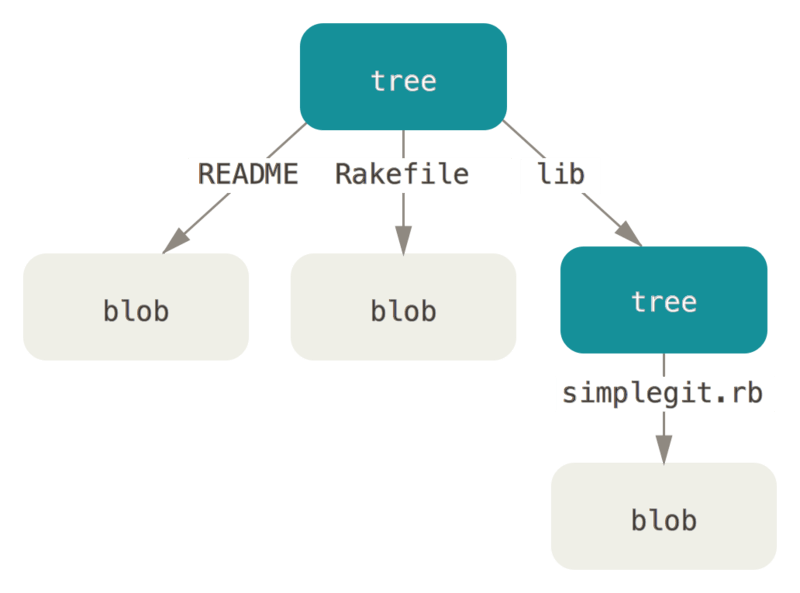
\includegraphics[width=0.5\textwidth]{gitTreeObject.png}
		\end{center}
\end{frame}

	\begin{frame}
		\frametitle{Какие ещё виды объектов бывают}
		\begin{center}
			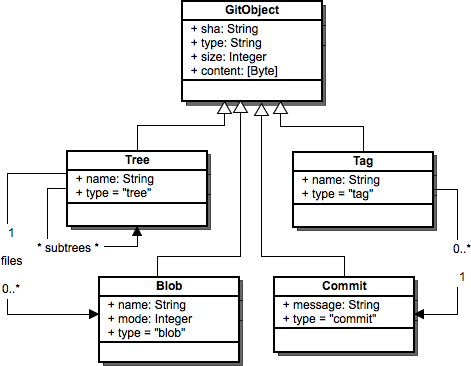
\includegraphics[width=0.7\textwidth]{gitDataStructure.png}
		\end{center}
	\end{frame}

	\begin{frame}[fragile]
		\frametitle{Коммиты}
		tree-объекты могут хранить структуру файлов (как inode в файловой системе), но не хранят метаинформацию типа автора файла и даты создания. Это хранится в commit-объектах:
		\begin{minted}{text}
$ echo 'first commit' | git commit-tree d8329f
fdf4fc3344e67ab068f836878b6c4951e3b15f3d

$ git cat-file -p fdf4fc3
tree d8329fc1cc938780ffdd9f94e0d364e0ea74f579
author Scott Chacon <schacon@gmail.com> 1243040974 -0700
committer Scott Chacon <schacon@gmail.com> 1243040974 -0700

first commit
		\end{minted}
		Ещё коммит хранит список коммитов-родителей
\end{frame}

	\begin{frame}
		\frametitle{Коммиты, как это выглядит}
		\begin{center}
			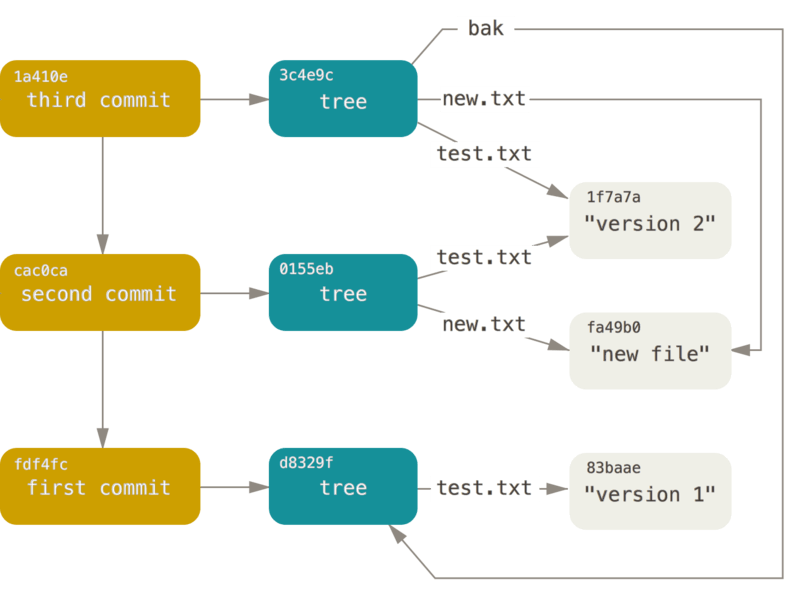
\includegraphics[width=0.7\textwidth]{gitCommitObjects.png}
		\end{center}
	\end{frame}

	\begin{frame}[fragile]
		\frametitle{Ссылки}
		Теперь вся информация хранится на диске, но чтобы ей воспользоваться, нужно помнить SHA-1 хеши. На помощь приходят reference-ы. 

		\begin{itemize}
			\item .git/refs
			\item .git/refs/heads
			\item .git/refs/tags
		\end{itemize}

		\begin{minted}{text}
$ echo "1a410efbd13591db07496601ebc7a059dd55cfe9" \
    > .git/refs/heads/master

$ git log --pretty=oneline master
1a410efbd13591db07496601ebc7a059dd55cfe9 third commit
cac0cab538b970a37ea1e769cbbde608743bc96d second commit
fdf4fc3344e67ab068f836878b6c4951e3b15f3d first commit
		\end{minted}
		\begin{itemize}
			\item Команда \verb|git update-ref|
		\end{itemize}
\end{frame}

	\begin{frame}
		\frametitle{Ссылки, как это выглядит}
		\begin{center}
			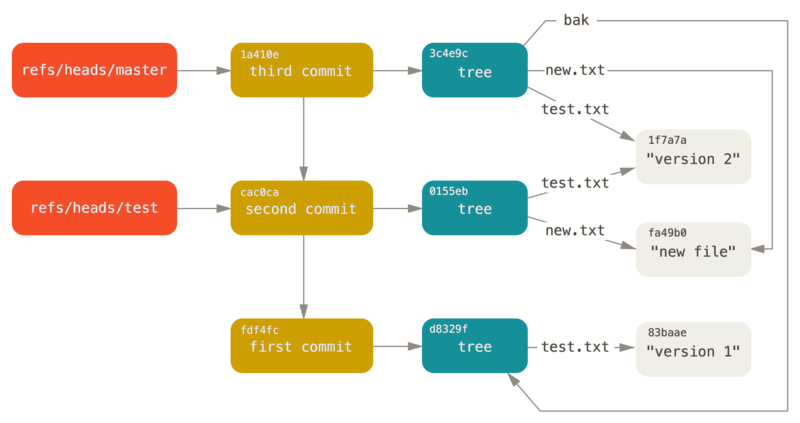
\includegraphics[width=0.9\textwidth]{gitRefs.png}
		\end{center}
	\end{frame}

	\begin{frame}[fragile]
		\frametitle{HEAD}
		Теперь не надо помнить хеши, но как переключаться между ветками?

		Текущая ветка хранится в HEAD. HEAD --- символическая ссылка, то есть ссылка на другую ссылку.
		\begin{minted}{text}
$ cat .git/HEAD
ref: refs/heads/master

$ git symbolic-ref HEAD refs/heads/test
$ cat .git/HEAD
ref: refs/heads/test
		\end{minted}
\end{frame}

	\begin{frame}[fragile]
		\frametitle{Тэги}
		Последний из объектов в Git --- tag. Это просто указатель на коммит.
		\begin{footnotesize}
			\begin{itemize}
				\item Легковесный тэг:
					\begin{minted}{text}
git update-ref refs/tags/v1.0 cac0cab538b970a37ea1e769cbbde608743bc96d
					\end{minted}
					Или просто git tag
				\item Аннотированный тэг:
					\begin{minted}{text}
$ git tag -a v1.1 1a410efbd13591db07496601ebc7a059dd55cfe9 -m 'test tag'

$ git cat-file -p 9585191f37f7b0fb9444f35a9bf50de191beadc2
object 1a410efbd13591db07496601ebc7a059dd55cfe9
type commit
tag v1.1
tagger Scott Chacon <schacon@gmail.com> Sat May 23 16:48:58 2009 -0700

test tag
					\end{minted}
			\end{itemize}
		\end{footnotesize}
\end{frame}

	\begin{frame}[fragile]
		\frametitle{Packfiles}
		Пока что получалось, что все версии всех файлов в Git хранятся целиком, как они есть. Все они всегда сжимаются zlib, но в целом, если создать репозиторий, добавлять туда файлы, коммитить и т.д., все версии всех файлов будут в нём целиком. На помощь приходят .pack-файлы:
		\begin{footnotesize}
			\begin{minted}{text}
$ git gc
Counting objects: 18, done.
Delta compression using up to 8 threads.
Compressing objects: 100% (14/14), done.
Writing objects: 100% (18/18), done.
Total 18 (delta 3), reused 0 (delta 0)

$ find .git/objects -type f
.git/objects/bd/9dbf5aae1a3862dd1526723246b20206e5fc37
.git/objects/d6/70460b4b4aece5915caf5c68d12f560a9fe3e4
.git/objects/info/packs
.git/objects/pack/pack-978e03944f5c581011e6998cd0e9e30000905586.idx
.git/objects/pack/pack-978e03944f5c581011e6998cd0e9e30000905586.pack
			\end{minted}
		\end{footnotesize}
\end{frame}

	\begin{frame}
		\frametitle{Как оно устроено}
		\begin{center}
			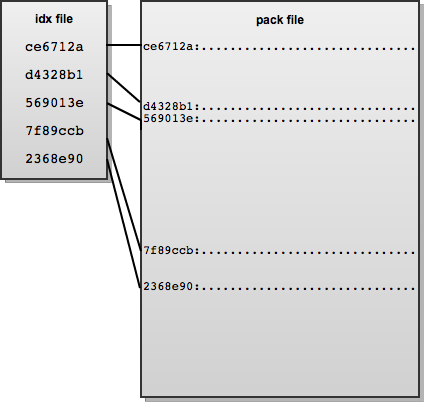
\includegraphics[width=0.6\textwidth]{gitPackFiles.png}
		\end{center}
	\end{frame}

	\begin{frame}
		\frametitle{Pack-файлы, подробности}
		\begin{itemize}
			\item Упаковка происходит, когда:
			\begin{itemize}
				\item Выполняется git push
				\item Слишком много <<свободных>> объектов (порядка 7000)
				\item Вручную вызвана git gc
			\end{itemize}
			\item Используется дельта-компрессия
			\begin{itemize}
				\item Последняя версия хранится целиком, дельты <<идут назад>>
			\end{itemize}
			\item Можно заглянуть внутрь, git verify-pack
			\item Git может хитро перепаковывать pack-файлы
		\end{itemize}
	\end{frame}

	\begin{frame}[fragile]
		\frametitle{Reflog и восстановление коммитов}
			\begin{minted}{text}
$ git reflog
1a410ef HEAD@{0}: reset: moving to 1a410ef
ab1afef HEAD@{1}: commit: modified repo.rb a bit
484a592 HEAD@{2}: commit: added repo.rb

$ git log -g
commit 1a410efbd13591db07496601ebc7a059dd55cfe9
Reflog: HEAD@{0} (Scott Chacon <schacon@gmail.com>)
Reflog message: updating HEAD
Author: Scott Chacon <schacon@gmail.com>
Date:   Fri May 22 18:22:37 2009 -0700

    third commit
$ git branch recover-branch ab1afef
			\end{minted}
\end{frame}

	\begin{frame}[fragile]
		\frametitle{Как более капитально прострелить себе ногу}
		\framesubtitle{И что делать}
		\begin{minted}{text}
$ git branch -D recover-branch
$ rm -Rf .git/logs/

$ git fsck --full
Checking object directories: 100% (256/256), done.
Checking objects: 100% (18/18), done.
dangling blob d670460b4b4aece5915caf5c68d12f560a9fe3e4
dangling commit ab1afef80fac8e34258ff41fc1b867c702daa24b
dangling tree aea790b9a58f6cf6f2804eeac9f0abbe9631e4c9
dangling blob 7108f7ecb345ee9d0084193f147cdad4d2998293
		\end{minted}
		Git не удалит даже <<висячие>> объекты несколько месяцев, если его явно не попросить.
\end{frame}

	\section{Задача}

	\begin{frame}
		\frametitle{Условие задачи}
		\framesubtitle{Своя локальная система контроля версий}
		Требуется сделать систему контроля версий, представляющую из себя консольное приложение и умеющую:
		\begin{itemize}
			\item commit с commit message (сообщение обязательно и принимается как параметр, система должна сама добавлять ещё дату коммита и автора)
			\item работу с ветками: создание и удаление
			\item checkout по имени ревизии или ветки
			\item log --- список ревизий вместе с commit message в текущей ветке
			\item merge --- сливает указанную ветку с текущей
			\begin{itemize}
				\item конфликты разрешайте (или не разрешайте) любым разумным способом
			\end{itemize}
		\end{itemize}
	\end{frame}

	\begin{frame}
		\frametitle{Нефункциональные требования}
		\begin{itemize}
			\item Документация: комментарии, помощь для пользователя, краткое описание внутреннего устройства
			\item Тесты
			\item Исключения, обработка ошибок
			\item Вывод в консоль --- только в клиентском коде типа main(), основной код должен позволять себя использовать как библиотеку
			\item Развитый программный интерфейс, должно быть можно без проблем потом прикрутить GUI
			\item Аннотации @NotNull, @Nullable/Optional
			\item Continuous Integration
		\end{itemize}
	\end{frame}

	\begin{frame}
		\frametitle{Примечания}
		\begin{itemize}
			\item Не накладывается никаких ограничений на хранимые на диске данные и их формат
			\begin{itemize}
				\item Дельта-компрессию делать не надо
			\end{itemize}
			\item Не требуется работа с удалёнными репозиториями
			\item Дедлайн: до 23:59 22.03
		\end{itemize}
	\end{frame}

\end{document}
